\ifdefined\handoutmode
  \PassOptionsToClass{handout}{beamer}
\fi
\documentclass[aspectratio=169]{beamer}

\input{../../../../hh_bpa_forel-preamble} % this is ugly.

\title{FMTS mätteknik HT2026 -- Dag 5}
\author{Pererik Andreasson \\ Struan Gray }
\date{\today{}}

% below is specific for the oscilloscope vs spectrum analyzer slides
% --- Colors -----------------------------------------------------------
\definecolor{slowc}{RGB}{40,110,220}   % slow wave
\definecolor{fastc}{RGB}{220,50,50}    % fast wave
\definecolor{tracec}{RGB}{255,210,40}  % oscilloscope trace
\definecolor{sqc}{RGB}{240,140,20}     % square wave

% --- Styles -----------------------------------------------------------
\pgfplotsset{
  % small plot without axes (for the "ingredients")
  mini/.style={
    width=3.2cm, height=2.0cm, axis lines=none,
    xmin=0, xmax=4*pi, ymin=-1.6, ymax=1.6,
    samples=200, domain=0:4*pi, scale only axis=false,
  },
  % instrument screen
  screen/.style={
    axis background/.style={fill=black!85},
    grid=major, grid style={green!35!black},
    xtick={0,1,...,10}, ytick={-2,-1,...,2},
    xticklabels={}, yticklabels={},
    major tick length=0pt,
    axis line style={black!60, line width=1.5pt},
    label style={font=\footnotesize},
    xlabel style={yshift=6pt}, ylabel style={yshift=-6pt},
  },
  timescreen/.style={
    screen, xmin=0, xmax=10, ymin=-2, ymax=2,
    xlabel={time $\rightarrow$}, ylabel={voltage},
    samples=300, domain=0:10,
  },
  freqscreen/.style={
    screen, xmin=0, xmax=10, ymin=-2, ymax=2,
    xlabel={frequency $\rightarrow$}, ylabel={level},
  },
  peak/.style={line width=3pt, mark=*, mark size=2.5pt, mark indices={2}},
}
% above is specific for the oscilloscope vs spectrum analyzer slides



\begin{document}

%%% Title slide: different footer, large logo
{
% no page #, no logo on title page
\setbeamertemplate{footline}{}
\setbeamertemplate{logo}{\titlelogos}
\begin{frame}
\vfill
  \begin{block}
    \maketitle
  \end{block}
\end{frame}
}


\frame{
    \frametitle{Lärandemål}
    {\Huge
    Nu är det prov!
    \begin{enumerate}
        \item<2-> \ldots
        \item<3-> \ldots
        \item<4-> \ldots
    \end{enumerate}
    }
}


\mode<beamer>{
\frame{
    \frametitle{Dagens plan}
    {\Large
        \begin{itemize}
            \item Mäta spänning på kondensator vid ''höga'' frekvenser.
            \item Närma oss gränserna för oscilloskopet - aliasfel och lite om upplösning.
            \item Vad är det med \qty{50}{\ohm}?
            \item begreppet decibel (och logaritmer)
            \item beräkna effekt på ingång
            \item använda power meter ($\times3$) - vi gör denna i par.
            \item Om tid finns: mäta längd på kabel, titta på reflektioner, titta i labbet
        \end{itemize}
    }
    }   
} % end mode


% Geometry used below:
%   signal:    3 periods, t = 0 ... 6*pi (18.8496), period 2*pi (6.2832)
%   box width: 4.0 for all six boxes
%   top:       starts 1.0, 6.0, 11.0         (spacing 5.0  != period)
%   bottom:    starts 0.5, 6.7832, 13.0664   (spacing 2*pi  = period)

% oscilloscope triggering example
\begin{frame}{Oscilloscope Triggering}
    \begin{figure}
        \centering

        % ---------------- Top: untriggered ----------------
        \begin{subfigure}[b]{\textwidth}
            \centering
            \begin{tikzpicture}
                \begin{axis}[
                    width=0.95\textwidth,
                    height=3.1cm,
                    axis lines=middle,
                    xlabel={$t$}, ylabel={$V$},
                    xlabel style={anchor=west},
                    ylabel style={anchor=south},
                    xtick=\empty, ytick=\empty,
                    xmin=0, xmax=18.8496, ymin=-1.4, ymax=1.4,
                    clip=false,
                ]
                    % three gray boxes, equal width, spacing 5.0 (not the period)
                    \filldraw[fill=shadecolor, draw=frameoff, dashed, thick]
                        (axis cs:1.0,-1.3)  rectangle (axis cs:5.0,1.3);
                    \filldraw[fill=shadecolor, draw=frameoff, dashed, thick]
                        (axis cs:6.0,-1.3)  rectangle (axis cs:10.0,1.3);
                    \filldraw[fill=shadecolor, draw=frameoff, dashed, thick]
                        (axis cs:11.0,-1.3) rectangle (axis cs:15.0,1.3);

                    % the signal (three full periods)
                    \addplot[sigcolor, thick, domain=0:18.8496, samples=300] {sin(deg(x))};

                    % start level of each box -- all different
                    \addplot[only marks, mark=*, mark size=2.2pt, frameoff]
                        expression[samples at={1.0,6.0,11.0}] {sin(deg(x))};
                \end{axis}
            \end{tikzpicture}
            \caption{Not triggered: each sweep starts at a different signal level.}
        \end{subfigure}

        \vspace{0.4cm}
\pause{}
        % ---------------- Bottom: triggered ----------------
        \begin{subfigure}[b]{\textwidth}
            \centering
            \begin{tikzpicture}
                \begin{axis}[
                    width=0.95\textwidth,
                    height=3.1cm,
                    axis lines=middle,
                    xlabel={$t$}, ylabel={$V$},
                    xlabel style={anchor=west},
                    ylabel style={anchor=south},
                    xtick=\empty, ytick=\empty,
                    xmin=0, xmax=18.8496, ymin=-1.4, ymax=1.4,
                    clip=false,
                ]
                    % three gray boxes, equal width, spacing = one period (2*pi)
                    \filldraw[fill=shadecolor, draw=frameon, dashed, thick]
                        (axis cs:0.5,-1.3)     rectangle (axis cs:4.5,1.3);
                    \filldraw[fill=shadecolor, draw=frameon, dashed, thick]
                        (axis cs:6.7832,-1.3)  rectangle (axis cs:10.7832,1.3);
                    \filldraw[fill=shadecolor, draw=frameon, dashed, thick]
                        (axis cs:13.0664,-1.3) rectangle (axis cs:17.0664,1.3);

                    % trigger level (sin(0.5) = 0.479)
                    \draw[dotted, thick, frameon]
                        (axis cs:0,0.479) -- (axis cs:18.8496,0.479);

                    % the signal (three full periods)
                    \addplot[sigcolor, thick, domain=0:18.8496, samples=300] {sin(deg(x))};

                    % start level of each box -- all the same
                    \addplot[only marks, mark=*, mark size=2.2pt, frameon]
                        expression[samples at={0.5,6.7832,13.0664}] {sin(deg(x))};
                \end{axis}
            \end{tikzpicture}
            \caption{Triggered: every sweep starts at the same level (dotted line).}
        \end{subfigure}

    \end{figure}
\end{frame}

% oscilloskoptriggeranteckningar
\handoutnoteslide

\begin{frame}
\frametitle{Problastning}
\resizebox{0.75\textwidth}{!}{%
\centering
    \begin{tikzpicture}[american]
        \ctikzset{bipoles/oscope/waveform=sin}
%        \ctikzset{bipoles/oscope/height=1.0}
        % ruta runt lågpassfiltret
        \draw[thick, gray, dashed] (1.25, 1.5) -- (1.25, 2.75) 
        -- (4.6, 2.75)
        -- (4.6, -0.25)
        -- (2.4, -0.25)
        -- (2.4, 1.5) -- cycle;
        
        % Signalkälla
        \draw (0, 0) node[ground, rotate=-90] {} to[sV, v<=\qty{1}{\V}, l_=\qty{2}{\MHz}, *-] (0, 2) ;
        % själva lågpassfiltret
        \draw (0, 2) -- (1, 2) to[R=\qty{1}{\kohm}] (3, 2)
                to[C=\qty{100}{\pF}] (3, 0) -- (0, 0) ;
        % Oscilloskop som mäter utgången över kondensatorn
        \draw (3, 2) -- (6, 2) to[oscope] (6, 0) node[ground]{};
        \draw [->, thick] (6, 1.5) -- (6, 2) -- (3, 2) ;
    \end{tikzpicture}
}
% resizebox
\centering
\\\vspace{3mm}
{\Large Mät $V_{PP}$ över kondensatorn med oscilloskopet.
    \\[3mm] (Fyll i tabellen på nästa bild.)
} % end large
\end{frame}

% tabell för mätresultat
\begin{frame}{Mätresultat.}
    \renewcommand{\arraystretch}{1.6} % more vertical breathing room
    \begin{table}
        \centering
        \begin{tabular}{
            >{\columncolor{firstcolcolor}\bfseries}l
            >{\centering\arraybackslash}c
            >{\centering\arraybackslash}c
            >{\centering\arraybackslash}c
            >{\centering\arraybackslash}c
        }
            \rowcolor{headercolor}
            \textcolor{white}{\textbf{Mät med:}} &
            \textcolor{white}{\textbf{Kroko/Bread}} &
            \textcolor{white}{\textbf{Prob/Bread}} &
            \textcolor{white}{\textbf{Kroko/Skruv}} &
            \textcolor{white}{\textbf{Prob/Skruv}} \\
            \midrule
            $V_{C}(PP)$ &  &  &  & \\
        \end{tabular}
    \end{table}
    \vspace{5cm}
\end{frame}



% upplösning - både horisontell och verikal
\begin{frame}
    \frametitle{Upplösning och digitalisering.}
    \resizebox{0.75\textwidth}{!}{
        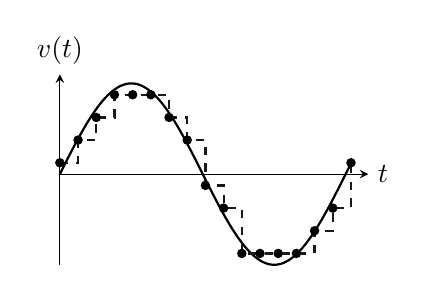
\begin{tikzpicture}
            \begin{axis}[
                width=55mm,
                height=40mm,
                axis lines=middle,
                xlabel={$t$},
                xlabel style={at={(axis description cs:1,0.475)},anchor=west},
                ylabel={$v(t)$},
                ylabel style={at={(axis description cs:0,1)},anchor=south},
                xmin=0, xmax=2*pi+0.5,
                ymin=-1, ymax=1.1,
                xtick=\empty,
                ytick=\empty,
                domain=0:2*pi+0.1,
                enlargelimits=false,
                clip=false,
                ]

                % -------- Parameters --------
                \pgfmathsetmacro{\A}{1}        % Full-scale amplitude
                \pgfmathsetmacro{\bits}{3}    % Bit resolution
                \pgfmathsetmacro{\L}{2^\bits} % Number of levels
                \pgfmathsetmacro{\Delta}{2*\A/\L}

                % -------- Analog signal --------
                \addplot[
                black,
                thick,
                samples=400,
                ]
                {sin(deg(x))};

                % -------- Sampled & quantized dots --------
                \addplot[
                only marks,
                mark=*,
                mark size=1.5pt,
                black,
                samples at={0,0.4,...,6.283},
                ]
                {
                    -\A
                    + \Delta * ( floor( ( sin(deg(x)) + \A ) / \Delta ) + 0.5 )
                };

                % -------- ZOH DAC output --------
                \addplot[
                black!90,
                dashed,
                thick,
                const plot,
                samples at={0,0.4,...,6.283},
                ]
                {
                    -\A
                    + \Delta * ( floor( ( sin(deg(x)) + \A ) / \Delta ) + 0.5 )
                };

                % -------- ZOH DAC output --------
                \addplot[
                black!90,
                dashed,
                thick,
                const plot,
                samples at={0,0.4,...,6.283},
                ]
                {
                    -\A
                    + \Delta * ( floor( ( sin(deg(x)) + \A ) / \Delta ) + 0.5 )
                };
            \end{axis}
        \end{tikzpicture}
    } % resizebox
\end{frame}

% aliasfel
\begin{frame}
    \frametitle{Aliasfel -- signaler med för hög frekvens. Skapa en sådan!}
    \resizebox{0.75\textwidth}{!}{
        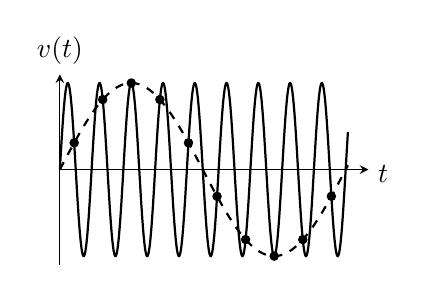
\begin{tikzpicture}
            \begin{axis}[
                width=55mm,
                height=40mm,
                axis lines=middle,
                xlabel={$t$},
                xlabel style={at={(axis description cs:1,0.475)},anchor=west},
                ylabel={$v(t)$},
                ylabel style={at={(axis description cs:0,1)},anchor=south},
                xmin=0, xmax=2*pi+0.5,
                ymin=-1.1, ymax=1.1,
                xtick=\empty,
                ytick=\empty,
                domain=0:2*pi+0.05,
                enlargelimits=false,
                clip=false,
                ]

                % High-frequency analog signal
                \addplot[
                black,
                thick,
                samples=600,
                ]
                {sin(deg(9*x))};

                % Low-frequency alias sine
                \addplot[
                black,
                thick,
                dashed,
                samples=600,
                ]
                {sin(deg(x))};

                % Dots at intersections of sin(9x) and sin(x)
                % sin(9x) = sin(x) => 9x = x + 2*pi*k or 9x = pi - x + 2*pi*k
                % => x = k*pi/4 or x = pi/10 + k*pi/5
                \addplot[
                only marks,
                mark=*,
                mark size=1.5pt,
                black,
                samples at={
                    0.3141592653589793,
                    0.9424777960769379,
                    1.5707963267948966,
                    2.199114857512855,
                    2.827433388230814,
                    3.455751918948772,
                    4.084070449666731,
                    4.71238898038469,
                    5.340707511102648,
                    5.969026041820607
                },
                ]
                {sin(deg(x))};
            \end{axis}
        \end{tikzpicture}
    } % resizebox
\end{frame}

\mode<beamer>{
\sectionslide{Nu blir det radio! (och logaritmer)}
} % end mode

\descriptionslide{figures/50ohm_siglent.png}{1}
    {Vad är det förresten som är \qty{50}{\ohm}?}
{
    \ringmarker{red}{0.715}{0.475}{1.2}
}

% 50 Ohm handout
\handoutnoteslide

\begin{frame}{Karakteristisk impedans -- repanalogin}
    \centering
    \begin{tikzpicture}[
        x=0.45cm, y=0.5cm,
        rope/.style={thick, ropecolor},
        heavyrope/.style={line width=2.5pt, ropecolor!70!black},
        move/.style={->, thick, movecolor},
        lbl/.style={anchor=east, align=right, font=\footnotesize},
        hdr/.style={font=\small\bfseries},
    ]
        % rubriker och avdelare
        \node[hdr] at (3.75,1.9)  {Före};
        \node[hdr] at (12.25,1.9) {Efter};
        \draw[gray!40] (8,1.6) -- (8,-8.3);

        % ---------- Rad 1: likadant rep = anpassad last ----------
        \begin{scope}
            \node[lbl] at (-0.4,0) {Likadant rep\\{\color{gray}anpassad last}};
            % före: puls på väg mot skarven
            \draw[rope] (0,0) -- plot[domain=0.7:2.3, samples=40]
                (\x,{0.4*(1+cos(225*(\x-1.5)))}) -- (7.5,0);
            \fill[ropecolor] (4.5,0) circle (2pt);
            \draw[move] (1.1,1.1) -- (1.9,1.1);
            % efter: pulsen har passerat skarven, ingen reflex
            \begin{scope}[shift={(8.5,0)}]
                \draw[rope] (0,0) -- plot[domain=5.2:6.8, samples=40]
                    (\x,{0.4*(1+cos(225*(\x-6)))}) -- (7.5,0);
                \fill[ropecolor] (4.5,0) circle (2pt);
                \draw[move] (5.6,1.1) -- (6.4,1.1);
            \end{scope}
        \end{scope}
\pause{}
        % ---------- Rad 2: fast vägg = kortslutning ----------
        \begin{scope}[shift={(0,-2.4)}]
            \node[lbl] at (-0.4,0) {Fast vägg\\{\color{gray}kortsluten ände}};
            % före
            \draw[rope] (0,0) -- plot[domain=0.7:2.3, samples=40]
                (\x,{0.4*(1+cos(225*(\x-1.5)))}) -- (4.5,0);
            \fill[pattern=north east lines, pattern color=gray] (4.5,-0.9) rectangle (5.1,0.9);
            \draw[very thick] (4.5,-0.9) -- (4.5,0.9);
            \draw[move] (1.1,1.1) -- (1.9,1.1);
            % efter: inverterad reflex
            \begin{scope}[shift={(8.5,0)}]
                \draw[rope] (0,0) -- plot[domain=0.7:2.3, samples=40]
                    (\x,{-0.4*(1+cos(225*(\x-1.5)))}) -- (4.5,0);
                \fill[pattern=north east lines, pattern color=gray] (4.5,-0.9) rectangle (5.1,0.9);
                \draw[very thick] (4.5,-0.9) -- (4.5,0.9);
                \draw[move] (1.9,1.1) -- (1.1,1.1);
            \end{scope}
        \end{scope}
\pause{}
        % ---------- Rad 3: fri ände = öppen ände ----------
        \begin{scope}[shift={(0,-4.8)}]
            \node[lbl] at (-0.4,0) {Fri ände\\{\color{gray}öppen ände}};
            % före
            \draw[gray, thick] (4.5,-0.9) -- (4.5,0.9);
            \draw[rope] (0,0) -- plot[domain=0.7:2.3, samples=40]
                (\x,{0.4*(1+cos(225*(\x-1.5)))}) -- (4.5,0);
            \draw[ropecolor, thick] (4.5,0) circle (2.5pt);
            \draw[move] (1.1,1.1) -- (1.9,1.1);
            % efter: reflex med samma tecken
            \begin{scope}[shift={(8.5,0)}]
                \draw[gray, thick] (4.5,-0.9) -- (4.5,0.9);
                \draw[rope] (0,0) -- plot[domain=0.7:2.3, samples=40]
                    (\x,{0.4*(1+cos(225*(\x-1.5)))}) -- (4.5,0);
                \draw[ropecolor, thick] (4.5,0) circle (2.5pt);
                \draw[move] (1.9,1.1) -- (1.1,1.1);
            \end{scope}
        \end{scope}
\pause{}
        % ---------- Rad 4: tyngre rep = felanpassning ----------
        \begin{scope}[shift={(0,-7.2)}]
            \node[lbl] at (-0.4,0) {Tyngre rep\\{\color{gray}felanpassning}};
            % före
            \draw[rope] (0,0) -- plot[domain=0.7:2.3, samples=40]
                (\x,{0.4*(1+cos(225*(\x-1.5)))}) -- (4.5,0);
            \draw[heavyrope] (4.5,0) -- (7.5,0);
            \draw[move] (1.1,1.1) -- (1.9,1.1);
            % efter: delvis reflex tillbaka, delvis vidare
            \begin{scope}[shift={(8.5,0)}]
                \draw[rope] (0,0) -- plot[domain=0.7:2.3, samples=40]
                    (\x,{-0.15*(1+cos(225*(\x-1.5)))}) -- (4.5,0);
                \draw[heavyrope] (4.5,0) -- plot[domain=5.4:6.6, samples=40]
                    (\x,{0.2*(1+cos(300*(\x-6)))}) -- (7.5,0);
                \draw[move] (1.9,1.1) -- (1.1,1.1);
                \draw[move] (5.6,1.1) -- (6.4,1.1);
            \end{scope}
        \end{scope}
    \end{tikzpicture}

    \vspace{2mm}
    {\footnotesize Repet = kabeln \quad Pulsen = signalen \quad Det som sitter i änden = lasten}
\end{frame}

% notes on the rope analogy
\handoutnoteslide

% Here inputing Emils frames (will recreate when I am not so tired)

% In preamble:
% \usepackage{pdfpages}

% In the document, OUTSIDE any frame environment:
\includepdf[pages=4]{emils_mtrl_pdf/Powermeter.pdf}

\handoutnoteslide

\mode<beamer>{
\sectionslide{Vad är dB? (Ja, logaritmer!)}
}

% dB bild
\includepdf[pages=8]{emils_mtrl_pdf/Powermeter.pdf}

\handoutnoteslide

\descriptionslide{uteffektlinear(1).png}{1}{}{}

\descriptionslide{uteffektdecibel(1).png}{1}{}{}

\begin{frame}{Räkneexempel: dBm}

\begin{block}{Definition}
\[
P_{\mathrm{dBm}} = 10\log_{10}\!\left(\frac{P}{1\,\mathrm{mW}}\right)
\qquad\Longleftrightarrow\qquad
P = 1\,\mathrm{mW}\cdot 10^{P_{\mathrm{dBm}}/10}
\]
\end{block}

\begin{columns}[T]
  \begin{column}{0.48\textwidth}
    \begin{exampleblock}{Exempel 1: W $\rightarrow$ dBm}
      En sändare ger $P = 2\,\mathrm{W}$.
    \mode<beamer>{
      \onslide<2->{
      \begin{align*}
        P &= 2\,\mathrm{W} = 2000\,\mathrm{mW}\\
        P_{\mathrm{dBm}} &= 10\log_{10}(2000)\\
                         &= 10 \cdot 3{,}30\\
                         &\approx \mathbf{33\,dBm}
      \end{align*}
      } % onslide
    } % end mode
    \end{exampleblock}
  \end{column}

  \begin{column}{0.48\textwidth}
    \begin{exampleblock}{Exempel 2: dBm $\rightarrow$ W}
      En mottagare mäter $P_{\mathrm{dBm}} = 17\,\mathrm{dBm}$.
    \mode<beamer>{
      \onslide<3->{
      \begin{align*}
        P &= 1\,\mathrm{mW}\cdot 10^{17/10}\\
          &= 10^{1{,}7}\,\mathrm{mW}\\
          &\approx 50\,\mathrm{mW}\\
          &= \mathbf{0{,}05\,W}
      \end{align*}
      } % onslide
    } % end mode
    \end{exampleblock}
  \end{column}
\end{columns}

\vspace{0.1cm}\mode<handout>{\vspace{3cm}}
\centering
\onslide<4->{
\small Tumregel: $+3\,\mathrm{dB} \approx 2\times$ effekten, \quad $+10\,\mathrm{dB} = 10\times$ effekten
}
\end{frame}

\handoutnoteslide

% dbuV räkneexempel
\begin{frame}{Räkneexempel: dB$\mu$V}

\begin{block}{Definition}
\[
U_{\mathrm{dB}\mu\mathrm{V}} = 20\log_{10}\!\left(\frac{U}{1\,\mu\mathrm{V}}\right)
\qquad\Longleftrightarrow\qquad
U = 1\,\mu\mathrm{V}\cdot 10^{U_{\mathrm{dB}\mu\mathrm{V}}/20}
\]
\end{block}

\begin{columns}[T]
  \begin{column}{0.48\textwidth}
    \begin{exampleblock}{Exempel 1: V $\rightarrow$ dB$\mu$V}
      En signal har spänningen $U = 10\,\mathrm{mV}$.
     \mode<beamer>{
      \onslide<2->{
      \begin{align*}
        U &= 10\,\mathrm{mV} = 10\,000\,\mu\mathrm{V}\\
        U_{\mathrm{dB}\mu\mathrm{V}} &= 20\log_{10}(10\,000)\\
                         &= 20 \cdot 4\\
                         &= \mathbf{80\,dB\boldsymbol{\mu}V}
      \end{align*}
      } % onslide
     } % end mode
    \end{exampleblock}
  \end{column}

  \begin{column}{0.48\textwidth}
    \begin{exampleblock}{Exempel 2: dB$\mu$V $\rightarrow$ V}
      En mottagare mäter $46\,\mathrm{dB}\mu\mathrm{V}$.
    \mode<beamer>{
      \onslide<3->{
      \begin{align*}
        U &= 1\,\mu\mathrm{V}\cdot 10^{46/20}\\
          &= 10^{2{,}3}\,\mu\mathrm{V}\\
          &\approx 200\,\mu\mathrm{V}\\
          &= \mathbf{0{,}2\,mV}
      \end{align*}
      } % onslide
    } % end mode
    \end{exampleblock}
  \end{column}
\end{columns}

\vspace{-0.5cm}\mode<handout>{\vspace{3cm}}
\centering
\onslide<4->{
\small Tumregel: $+6\,\mathrm{dB} \approx 2\times$ spänningen, \quad $+20\,\mathrm{dB} = 10\times$ spänningen\\[2pt]
I $50\,\Omega$: \quad $U_{\mathrm{dB}\mu\mathrm{V}} \approx P_{\mathrm{dBm}} + 107$
} % onslide
\end{frame}

\handoutnoteslide

\mode<beamer>{
\sectionslide{Egentligen är dB bara till för att ingenjörer inte vill \textit{räkna någt}.}
}

\includepdf[pages=11]{emils_mtrl_pdf/Powermeter.pdf}

\handoutnoteslide

\includepdf[pages=6]{emils_mtrl_pdf/Powermeter.pdf}

\handoutnoteslide


\includepdf[pages=16]{emils_mtrl_pdf/Powermeter.pdf}

\handoutnoteslide

% ======================================================================
\begin{frame}{Same signal -- two ways to look at it}

\centering
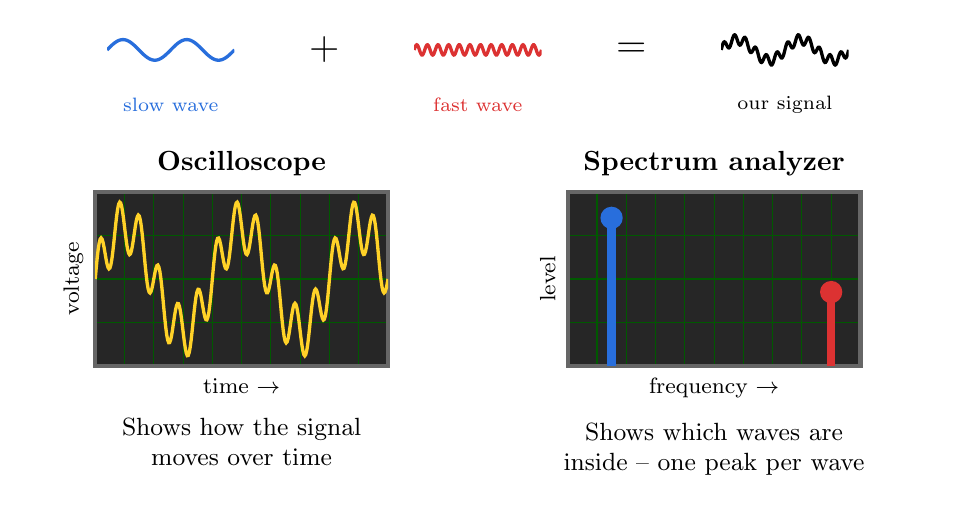
\begin{tikzpicture}

  % ---- Top: the signal is made of two "ingredients" ------------------
  \begin{axis}[mini, name=slow, at={(0cm,0cm)}, anchor=center]
    \addplot[slowc, very thick] {sin(deg(x))};
  \end{axis}
  \node[font=\Large\bfseries] at (1.95,0) {$+$};
  \begin{axis}[mini, name=fast, at={(3.9cm,0cm)}, anchor=center]
    \addplot[fastc, very thick] {0.5*sin(deg(6*x))};
  \end{axis}
  \node[font=\Large\bfseries] at (5.85,0) {$=$};
  \begin{axis}[mini, name=sum, at={(7.8cm,0cm)}, anchor=center]
    \addplot[black, very thick] {sin(deg(x)) + 0.5*sin(deg(6*x))};
  \end{axis}
  \node[font=\scriptsize, slowc] at (0,-0.7) {slow wave};
  \node[font=\scriptsize, fastc] at (3.9,-0.7) {fast wave};
  \node[font=\scriptsize]        at (7.8,-0.7) {our signal};

  % ---- Bottom: the two instruments -----------------------------------
  \begin{axis}[timescreen, name=scope, width=5.3cm, height=3.8cm,
               at={(0.9cm,-1.8cm)}, anchor=north,
               title={\textbf{Oscilloscope}}, title style={yshift=-4pt}]
    \addplot[tracec, very thick]
      {1.2*sin(deg(0.5*pi*x)) + 0.6*sin(deg(3*pi*x))};
  \end{axis}

  \begin{axis}[freqscreen, name=sa, width=5.3cm, height=3.8cm,
               at={(6.9cm,-1.8cm)}, anchor=north,
               title={\textbf{Spectrum analyzer}}, title style={yshift=-4pt}]
    \addplot[peak, slowc] coordinates {(1.5,-2) (1.5,1.4)};
    \addplot[peak, fastc] coordinates {(9,-2) (9,-0.3)};
  \end{axis}

  % ---- One-line captions ---------------------------------------------
  \node[font=\small, text width=5.2cm, align=center, below=2pt, execute at begin node={\hyphenpenalty=10000}]
    at (scope.below south) {Shows \alert{how the signal moves} over time};
  \node[font=\small, text width=5.2cm, align=center, below=2pt, execute at begin node={\hyphenpenalty=10000}]
    at (sa.below south) {Shows \alert{which waves} are inside -- one peak per wave};

\end{tikzpicture}

\end{frame}

% ======================================================================
\begin{frame}{Examples}

\centering
\begin{tikzpicture}
  \pgfplotsset{
    ex/.style={scale only axis, width=4.0cm, height=1.5cm, xlabel={}, ylabel={}},
  }

  % column headers
  \node[font=\bfseries\small] at (3.3,0.35) {Oscilloscope};
  \node[font=\bfseries\small] at (8.6,0.35) {Spectrum analyzer};
  \node[font=\scriptsize, black!60] at (3.3,0.0)  {time $\rightarrow$};
  \node[font=\scriptsize, black!60] at (8.6,0.0)  {frequency $\rightarrow$};

  % ---- Row 1: one tone -------------------------------------------------
  \node[font=\small, align=center] at (0,-1.1) {One\\tone};
  \begin{axis}[timescreen, ex, at={(3.3cm,-1.1cm)}, anchor=center]
    \addplot[slowc!60!white, very thick] {1.3*sin(deg(pi*x))};
  \end{axis}
  \draw[-{Stealth}, very thick, black!40] (5.55,-1.1) -- (6.35,-1.1);
  \begin{axis}[freqscreen, ex, at={(8.6cm,-1.1cm)}, anchor=center]
    \addplot[peak, slowc!60!white] coordinates {(3,-2) (3,1.3)};
  \end{axis}

  % ---- Row 2: two tones ------------------------------------------------
  \node[font=\small, align=center] at (0,-3.3) {Two\\tones};
  \begin{axis}[timescreen, ex, at={(3.3cm,-3.3cm)}, anchor=center]
    \addplot[tracec, very thick]
      {1.1*sin(deg(0.5*pi*x)) + 0.6*sin(deg(3*pi*x))};
  \end{axis}
  \draw[-{Stealth}, very thick, black!40] (5.55,-3.3) -- (6.35,-3.3);
  \begin{axis}[freqscreen, ex, at={(8.6cm,-3.3cm)}, anchor=center]
    \addplot[peak, slowc] coordinates {(1.5,-2) (1.5,1.3)};
    \addplot[peak, fastc] coordinates {(9,-2) (9,-0.3)};
  \end{axis}

  % ---- Row 3: square wave ---------------------------------------------
  \node[font=\small, align=center] at (0,-5.5) {Square\\wave};
  \begin{axis}[timescreen, ex, at={(3.3cm,-5.5cm)}, anchor=center, samples=801]
    \addplot[sqc, very thick] {sin(deg(0.5*pi*x)) >= 0 ? 1.3 : -1.3};
  \end{axis}
  \draw[-{Stealth}, very thick, black!40] (5.55,-5.5) -- (6.35,-5.5);
  \begin{axis}[freqscreen, ex, at={(8.6cm,-5.5cm)}, anchor=center]
    \foreach \n in {1,3,5,7,9} {
      \pgfmathsetmacro\h{-2+3.3/\n}
      \edef\temp{\noexpand\addplot[peak, sqc, line width=2.5pt]
        coordinates {(\n,-2) (\n,\h)};}
      \temp
    }
  \end{axis}

\end{tikzpicture}

\end{frame}


\instructionslide{Här kördes lite demo på spektrumanalysatorn. Det går inte att hinna med power meter på riktigt på en timme utan att det blir demo. Hur förbereder man olika grupper? Eller skall vi köra Mini circuits?}

\begin{frame}{What should the power meter show?}

\begin{columns}[c]

% ---- Left: simple circuit ------------------------------------------------
\begin{column}{0.37\textwidth}
\centering
\begin{tikzpicture}[thick, font=\small, scale=0.9, transform shape]
  % generator (dashed outline)
  \draw[dashed, rounded corners=3pt] (-0.9,-1.5) rectangle (1.9,1.6);
  \node[above] at (0.5,1.6) {Function generator};

  % sine source
  \draw (0,-1) -- (0,-0.4);
  \draw (0,0) circle (0.4);
  \draw (-0.25,0) sin (-0.125,0.15) cos (0,0) sin (0.125,-0.15) cos (0.25,0);
  \draw (0,0.4) -- (0,1) -- (0.6,1);

  % internal 50 ohm
  \draw (0.6,0.85) rectangle (1.4,1.15);
  \node[above, font=\scriptsize] at (1.0,1.15) {$50\,\Omega$};
  \draw (1.4,1) -- (3.2,1);
  \draw (0,-1) -- (3.2,-1);

  % meter = 50 ohm load
  \draw (3.05,0.4) rectangle (3.35,-0.4);
  \draw (3.2,1) -- (3.2,0.4);
  \draw (3.2,-0.4) -- (3.2,-1);
  \node[left, font=\scriptsize] at (3.05,0) {$50\,\Omega$};
  \node[below, align=center] at (3.2,-1.5) {Power meter /\\spectrum analyzer};

  % voltage across the load
  \draw[-{Stealth}] (3.8,-0.7) -- (3.8,0.7);
  \node[right, font=\scriptsize] at (3.8,0) {$\hat U = 2\,\mathrm{V}$};
\end{tikzpicture}
\end{column}

% ---- Right: the math -----------------------------------------------------
\begin{column}{0.61\textwidth}
\begin{align*}
  \hat U &= 2\,\mathrm{V}
    \quad \text{\scriptsize (amplitude, $4\,\mathrm{V_{pp}}$)}\\[4pt]
  U_{\mathrm{rms}} &= \frac{\hat U}{\sqrt 2} \approx 1{.}41\,\mathrm{V}
    \quad \text{\scriptsize (sine)}\\[4pt]
  P &= \frac{U_{\mathrm{rms}}^2}{R} = \frac{1{.}41^2}{50} = 40\,\mathrm{mW}\\[4pt]
  P_{\mathrm{dBm}} &= 10\log_{10}\!\left(\frac{40\,\mathrm{mW}}{1\,\mathrm{mW}}\right)
    \approx \boxed{16\,\mathrm{dBm}}
\end{align*}

\vspace{2pt}
{\scriptsize
Generator set to \textbf{50\,\boldmath$\Omega$ load}: the 2\,V is what
actually reaches the meter.\\[2pt]
Set to \textbf{High-Z} instead? Only half the voltage reaches the meter
$\Rightarrow$ $-6\,\mathrm{dB}$ $\Rightarrow$ \textbf{10\,dBm}.
}
\end{column}

\end{columns}

\end{frame}

\handoutnoteslide

\includepdf[pages=2]{emils_mtrl_pdf/Powermeter.pdf}

\handoutnoteslide

\includepdf[pages=15]{emils_mtrl_pdf/Powermeter.pdf}

\handoutnoteslide

\begin{frame}{Speed of light in a coaxial cable}

\centering
\begin{tikzpicture}[
    box/.style={draw, thick, rounded corners=2pt},
    cable/.style={line width=1.4pt},
    jack/.style={circle, draw, thick, fill=white, inner sep=1.6pt},
    lbl/.style={font=\small},
  ]

  % ---- Function generator ---------------------------------------------
  \draw[box] (0,0) rectangle (2.4,1.6);
  \node[lbl, above] at (1.2,1.6) {Function generator};
  % pulse symbol
  \draw[thick] (0.4,0.5) -- (0.9,0.5) -- (0.9,1.1) -- (1.3,1.1)
               -- (1.3,0.5) -- (2.0,0.5);
  \node[font=\scriptsize, below] at (1.2,0.45) {short pulse};
  \node[jack] (out) at (2.4,0.8) {};

  % ---- T-connector ----------------------------------------------------
  \fill (3.2,0.8) circle (2.5pt);
  \draw[cable] (out) -- (3.2,0.8);

  % ---- Oscilloscope ---------------------------------------------------
  \draw[box] (6,-0.8) rectangle (10.6,3.0);
  \node[lbl, above] at (8.3,3.0) {Oscilloscope};
  \node[jack] (ch1) at (6,2.0) {};
  \node[jack] (ch2) at (6,0.2) {};
  \node[font=\scriptsize, right] at (6.1,2.0) {CH1};
  \node[font=\scriptsize, right] at (6.1,0.2) {CH2};

  % screen (white, light grid)
  \draw[thick] (7.0,-0.5) rectangle (10.3,2.7);
  \draw[black!20, step=0.4, shift={(7.0,-0.5)}]
    (0,0) grid (3.3,3.2);

  % CH1 trace: pulse directly from the generator
  \draw[very thick] (7.0,1.8) -- (7.6,1.8) -- (7.6,2.35) -- (7.95,2.35)
                    -- (7.95,1.8) -- (10.3,1.8);
  % CH2 trace: same pulse, delayed by the cable
  \draw[very thick] (7.0,0.0) -- (9.1,0.0) -- (9.1,0.5) -- (9.45,0.5)
                    -- (9.45,0.0) -- (10.3,0.0);

  % delay marker
  \draw[dashed] (7.6,-0.5) -- (7.6,2.7);
  \draw[dashed] (9.1,-0.5) -- (9.1,2.7);
  \draw[{Stealth}-{Stealth}, thick] (7.6,1.05) -- (9.1,1.05)
    node[midway, fill=white, inner sep=1.5pt] {$\Delta t$};

  % ---- Cables ---------------------------------------------------------
  % short cable -> CH1
  \draw[cable] (3.2,0.8) |- (ch1);
  % long coax (coiled) -> CH2
  \draw[cable] (3.2,0.8) -- (3.2,-1.3);
  \draw[cable, decorate,
        decoration={coil, aspect=0.6, segment length=3.2mm, amplitude=4mm,
                    pre length=0.2cm, post length=0.2cm}]
    (3.2,-1.3) -- (5.3,-1.3);
  \draw[cable] (5.3,-1.3) -- (5.6,-1.3) |- (ch2);
  \node[lbl, below] at (4.25,-1.75) {long coax, length $L$};

  % ---- Formula --------------------------------------------------------
  \node[draw, thick, inner sep=6pt, font=\Large] at (12.4,1.3)
    {$v = \dfrac{L}{\Delta t}$};
  \node[font=\scriptsize] at (12.4,0.25) {(typically $v \approx \tfrac{2}{3}\,c$)};

\end{tikzpicture}

\end{frame}


\handoutnoteslide


\mode<beamer>{\finalslide}

\end{document}
